
\section{Contextualização}\label{sec:contexto}


Para lidar com mudanças e crescentes necessidades de negócios, sistemas de software estão em constante evolução. Atividades de evolução do software podem abranger desde a manutenção até a substituição total do sistema~\cite{seacord_2003}. De acordo com~\citeonline{Lientz_1978} a manutenção de software é a atividade mais custosa no ciclo de vida do sistema de software. O processo de manutenção de software inclui um conjunto de tarefas necessárias para modificar o software existente, e ainda deve-se preservar sua integridade. As tarefas de manutenção de software podem ser vistas como modificações incrementais que adicionam ou atualizam um conjunto de funcionalidades, ou corrigem falhas do projeto. Usualmente, com o passar do tempo, a integridade conceitual do sistema tende a diminuir, o que afeta a sua qualidade. Essa deterioração é conhecida na literatura como o fenômeno de envelhecimento~\cite{Fowler1999}, lidar com esse fenômeno não é uma atividade trivial e barata.

Uma técnica comum e amplamente utilizada para lidar com este problema é a aplicação de um processo de reestruturação de software com o intuito de melhorar sua estrutura e o seu \emph{design}. O processo de reestruturação de software que segue o paradigma orientado a objeto é comumente chamado de refatoração~\cite{OPDYKE_1992, Fowler1999, Mens04}. A refatoração foi primeiramente proposta por~\citeonline{OPDYKE_1992} como uma metodologia para reestruturar programas. Seguindo a mesma linha de pensamento, pesquisadores como o \citeonline{Fowler1999} tornaram a refatoração uma disciplina comumente conhecida e aplicada. A refatoração é um processo disciplinado que é utilizado para melhorar a estrutura de software, preservando seu comportamento~\cite{Fowler1999}. Com o apoio ferramental adequado, a refatoração pode ser uma maneira eficiente e eficaz para ajudar a melhorar o \emph{design} do software, tornar o software mais fácil de entender, e para auxiliar na identificação de erros. %Na literatura é possível identificar um conjunto de ferramentas, automáticas ou semiautomáticas, que auxiliam na aplicação de refatorações (refs). 


Outra linha de pesquisa que vem se popularizando é a Engenharia Dirigida por Modelos (do inglês - \sigla{MDD}{\textit{Model-Driven Development}}). Usualmente, pesquisas encontradas na literatura sobre refatorações estão mais focadas em criar ferramentas e abordagens para refatorações que ocorrem em nível de código-fonte. No entanto, com o surgimento da MDD aumentou o interesse e a necessidade de ferramentas de apoio à refatorações em nível de modelo. Na verdade, de acordo com~\citeonline{Mens_and_Tourwe_2004} a adaptação de ferramentas de refatoração para fornecer apoio à aplicação de refatorações em nível de modelo pode ser de grande utilidade. Algumas motivações podem ser destacadas para a realização dessas adaptações: (\emph{i}) modelos podem fornecer uma visão abstrata do sistema; assim, visualizações de mudanças estruturais são mais fáceis de serem visualizadas e detectadas; (\emph{ii}) problemas descoberto ainda em nível de \emph{design} podem ser solucionados diretamente no modelo aumentando a produtividade; e (\emph{iii}) a capacidade de explorar caminhos alternativos de decisões é muito mais barato em nível de modelo, uma vez que não se faz necessário a alteração direta do código-fonte, fazendo com que o sistema ainda opere enquanto mudanças são testadas pelo modernizador.


O processo de refatorações em nível de modelos tende a ser mais complexo do que refatorações aplicadas em código-fonte~\cite{Mens_2006}, uma vez que além das refatorações é necessária também a realização de atividades para verificar a consistência do modelo, manter a sincronização do modelo e suas visões, etc~\cite{KolahdouzRahimi20145}. Segundo~\citeonline{Gorp}, desenvolvedores de software utilizam refatorações em nível de \emph{design}, assim, é intuitivo explorar os conceitos de MDD utilizando a UML para a aplicação de refatorações~\cite{Salem_2008, Gorp, Egyed_2008, Briand_2006, staron2004implementing}. Nesse sentido, vários pesquisadores iniciaram pesquisas com o objetivo de implementar refatorações no contexto da UML~\cite{revisao_sistematica_uml_refactoring}. Uma das vantagens em se utilizar refatorações em nível de modelos, tais como a UML, é que os desenvolvedores de software não precisam se preocupar com características especificas de linguagens de programação (Java, C++, C\#, etc). Além disso, a utilização de um diagrama de classe fornece uma visão abstrata do sistema, assim, o engenheiro pode facilmente visualizar e verificar quais refatorações devem ser aplicadas no sistema. 

No entanto, de acordo com~\citeonline{Gorp} utilizar apenas os diagramas da UML não é uma abordagem adequada para manter e representar todos os artefatos de um sistema de software. Isso ocorre principalmente porque a UML não consegue representar todas as construções de um determinado sistema, por exemplo, declarações internas de um método não são consideradas no contexto do metamodelo da UML. Além disso, a UML não contém um conjunto de metaclasses para representar todos os artefatos de um sistema. Com a UML não é possível representar níveis mais baixos de abstração de um sistema, como o código-fonte, nem mesmo representar níveis mais altos, como a arquitetura do sistema e regras de negócios. Utilizando o metamodelo da UML poucas informações do código-fonte são representadas, por exemplo, nome da classe, nome do método e seus parâmetros, atributos e seus tipos.  

Com o objetivo de mitigar essa limitação em 2003 o \textit{Object Management Group} (OMG) criou uma força tarefa para analisar e evoluir os tradicionais processos de reengenharia, formalizando-os e fazendo com que eles fossem totalmente apoiados por modelos~\cite{ADM:OMG}. Logo, o termo Modernização Dirigida à Arquitetura (do inglês - \sigla{ADM}{\textit{Architecture-Driven Modernization}}) surgiu como uma solução para os problemas de padronização. A ADM é um processo de modernização de sistemas legados que utiliza um conjunto de metamodelos para representar completamente um sistema por meio de diferentes representações arquiteturais. Esses modelos são então submetidos à refatorações, otimizações e posteriormente o código-fonte pode ser então gerado novamente por meio de atividades de engenharia avante. Durante a modernização de um sistema são gerados vários modelos de acordo com os metamodelos da ADM, que representam diferentes partes/visões do sistema, como: fluxo de dados, banco de dados, elementos de programação (métodos, classes, tipos de dados, etc.) e arquitetura~\cite{PerezCastillo20121370}.

O Knowledge Discovery Metamodel (KDM) é o principal metamodelo da ADM com uma ampla quantidade de metaclasses para representar desde os níveis mais baixos de abstração de um sistema (código-fonte), até níveis mais altos (arquitetura do sistema), permitindo a representação de conceitos de qualquer domínio~\cite{KDM:specification,KDM:ISO}. Diferentemente de metamodelos existentes, como a UML, o KDM mantêm todas as visões/representações do sistema em uma única instância do KDM; o KDM pode ser considerado como uma família de metamodelos, uma vez que o mesmo compartilha a consistência e terminologia homogenia. A ideia principal da ADM é que a comunidade comece a desenvolver ferramentas que atuem apenas sobre instancias do metamodelo KDM, ao invés de serem dependentes de plataformas e linguagens especificas. Por exemplo, um catálogo de refatorações~\cite{durelli_catalogo} para o KDM tem o poder de reestruturar um sistema independentemente da linguagem de programação que foi usada em seu desenvolvimento, já que as refatorações ocorrem nos modelos. Outro exemplo seria a aplicação de técnicas de mineração de interesses transversais utilizando como base o metamodelo KDM~\cite{Durelli:2013_ACM, dani_san, daniel_san_journal}.


No entanto, embora a ADM tenha investido esforços para fornecer metamodelos para auxiliar o engenheiro de modernização a conduzir a reengenharia de um sistema seguindo todas as diretrizes de MDD, a ADM ainda não fornece instruções de como criar, reusar e/ou aplicar refatorações no metamodelo KDM, nem mesmo como manter uma determinada instância do KDM sincronizada após a aplicação de refatorações. Assim, tais particularidades devem ser tratadas pelos engenheiros de modernização. Isto faz com que os engenheiros criem suas próprias soluções. Porém, usualmente tais soluções são proprietárias e especificas o que pode dificultar a interoperabilidade entre diferentes soluções. Dessa forma, nesta Tese é apresentada uma abordagem para criação e disponibilização de refatorações para o metamodelo KDM, bem como um apoio ferramental que permite aplicá-las em diagramas de classe da UML. 

%Esta tese de doutorado aborda as seguintes questões de pesquisas (QP):

%\begin{itemize}
% 	\item \textbf{QP$_1$}: Qual é o estado da arte de refatorações no contexto da ADM, e principalmente para o metamodelo KDM?;
% 	\item \textbf{QP$_2$}: Como manter todas as visões do metamodelo KDM sincronizado após a aplicação de um conjunto de refatorações?;
 %	\item \textbf{QP$_3$}: Como especificar refatorações para que elas possam ser disponibilizadas/reutilizadas de forma independente de linguagem e plataforma de programação?;
 %	\item \textbf{QP$_4$}: Como automatizar o processo de aplicação de refatorações dentro do contexto da ADM e KDM?.
 %\end{itemize} 


\section{Motivações}\label{sec:justificativa_e_motivacao}

%Refatorações são técnicas utilizadas para melhorar a estrutura do software~\cite{Fowler1999}. Hoje em dia é evidente que a refatoração é de suma importância para melhorar a qualidade do código-fonte. Embora a refatoração para modelos tenha alcançado bastante reconhecimento e aceitação~\cite{Salem_2008, Gorp, Egyed_2008, Briand_2006, staron2004implementing}, ainda se faz necessárias pesquisas nessa área~\cite{revisao_sistematica_uml_refactoring, durelli_systematic_mapping}. 

%Embora a ADM e o KDM tenham sido propostos para auxiliar todo o processo da modernização de sistemas por meio de modelos, ainda hoje existe uma ausência de abordagens e apoios computacionais para auxiliar os engenheiros de modernização durante a aplicação de refatorações de forma consistente em instâncias do metamodelo KDM\footnote{É importante ressaltar que para facilitar a leitura e o entendimento  desta Tese em vários pontos o termo \aspas{refatorações para o KDM} será utilizada de forma intercambiável a \aspas{refatorações aplicadas em instâncias do metamodelo KDM}.}. Dessa forma, usualmente os engenheiros de modernização precisam desenvolver suas próprias abordagens e apoios ferramentais para refatorar diversos sistemas. Tais soluções tendem a ser proprietárias e consequentemente tornam-se difíceis de serem reutilizadas e dificulta a interoperabilidade entre outras ferramentas. Assim, é possível concluir que este é um campo atual e promissor para novas pesquisas. Nesse contexto, a pesquisa apresentada nesta tese visa a contribuir para a criação de abordagens e apoios computacionais para auxiliar os engenheiros de software durante a aplicação de refatorações para o KDM. No contexto desta Tese, as principais motivações são:

As motivações que levaram ao desenvolvimento desta Tese foram:

\begin{enumerate}

\item A escassez de abordagens para criar refatorações para o KDM. Isto é, quais são as diretrizes que permitem o engenheiro de modernização criar refatorações tradicionais para o metamodelo KDM. A ausência de diretrizes desse tipo dificulta a criação de refatorações para o KDM, fazendo com que engenheiros de modernização tenham que criar suas próprias soluções;

\item Ausência de uma infraestrutura de suporte ao reúso de refatorações para o KDM. A ausência de uma infraestrutura desse tipo faz com que engenheiros de modernização criem suas próprias soluções para especificar, armazenar e disponibilizar refatorações, dificultando bastante o reúso delas em outros contextos. 



%\item Ausência de um metamodelo que reúna as principais informações relacionadas com refatorações. Refatorações são disponibilizadas por meio de linguagem natural~\cite{Fowler1999}, porém não são facilmente reutilizadas. Uma abordagem promissora é lidar com a refatoração de forma independente da linguagem – aumentando assim as possibilidades de reutilização das refatorações;

%\item Embora a ADM forneça um conjunto de metamodelos para auxiliar o engenheiro de modernização a conduzir modernização até esse momento a ADM não provê instruções para auxiliar o engenheiro a promover o reúso de refatorações juntamente com os seus metamodelos padronizados (por exemplo, KDM) durante o processo de modernização. Essa limitação faz com que o engenheiro de modernização crie suas próprias soluções/refatorações, resultando em um possível atraso no processo de modernização. Contudo, as soluções/refatorações  definidas não são facilmente reutilizadas, pois tendem a ser proprietárias e específicas de linguagem e plataforma. Uma solução promissora é lidar com a refatoração de forma independente da linguagem – aumentando assim as possibilidades de reutilização de refatorações. Dessa forma, existe a motivação de criar uma metamodelo para auxiliar o engenheiro de modernização a promover o reúso de refatorações no contexto da ADM e principalmente de forma integrada com o metamodelo KDM. 


\item Carência de apoios computacionais efetivos para auxiliar o engenheiro de software durante a aplicação, disponibilização e reúso de refatorações para o KDM. A escassez de apoio computacional efetivo pode também dificultar a condução adequada de refatorações para o KDM.

\end{enumerate}

Nesse contexto, a pesquisa apresentada nesta tese visa a contribuir para a definição de uma abordagem para a criação, disponibilização e aplicação de refatorações para o KDM.


%É comumente observado que a atividade de refatoração é pertinente a qualquer processo de modernização. Dessa forma, quando um sistema é representado utilizando diferentes visões conceituais para representar níveis de abstração do sistema (por exemplo, visão arquitetural, visão de código-fonte, visão do banco de dados, etc), um acidente comum que surge durante atividades de refatorações é a dessincronização das instâncias do metamodelo, resultando em visões inconsistente após a aplicação de uma refatoração. Dessa forma, no contexto do metamodelo KDM existe uma carência em abordagens e ferramentas que auxiliam a sincronizar tais mudanças após a aplicação de um conjunto de refatorações no KDM. Pesquisas recentes sugerem que a aplicação de técnicas de propagação de mudanças podem auxiliar na identificação e atualização de todas as instâncias/visões do KDM, permitindo assim manter todas as visões/instâncias do metamodelo KDM sincronizadas [7]–[10]. 
%Usualmente, o processo de refatorações em modelos é mais complexo do que refatoções em código-fonte (ref), uma vez que além das refatorações é necessário também a realização de atividades para verificar a consistência do modelo, manter a sincronição do modelo e suas visões, etc. Em consequência disso, poucos avanços significativos foram conseguidos em relação a definição de refatoração para o metamodelo KDM.
%
%Pode-se destacar as principais motivações para aplicar refatorações em nível de modelos, principalmente utilizando o KDM:

%\begin{itemize}

    %\item Embora a refatoração para modelos tenha alcançado bastante reconhecimento e aceitação, até o presente momento apenas trabalhos desenvolvido no contexto do metamodelo \sigla{UML}{\textit{Unified Modeling Language}} foram encontrados e consolidados na literatura~\cite{revisao_sistematica_uml_refactoring, durelli_systematic_mapping}. 
    
 %   \item Ausência de abordagens para adaptar e especificar refatorações para o KDM. %Até o presente momento apenas trabalhos desenvolvidos no contexto metamodelo \sigla{UML}{\textit{Unified Modeling Language}} foram encontrados e consolidados na literatura~\cite{revisao_sistematica_uml_refactoring, durelli_systematic_mapping}. Neste contexto, existe uma motivação para criar diretrizes de como adaptar refatorações para o KDM.
    
    %Dessa forma, existe uma ausência de abordagens para o metamodelo KDM, uma vez que o mesmo é um metamodelo mais novo quando comparado a UML. A refatoração de um sistema em geral tende a ser uma atividade complexa; modificações manuais, sem qualquer catálogo de refatoração, bem como um ambiente integrado, pode resultar em efeitos colaterais indesejados e acarretar em um processo tedioso. Neste contexto, existe uma necessidade para elaborar/adaptar um catálogo de refatoração para o metamodelo KDM e também criar um ambiente que auxilie a aplicação de refatorações diretamente no KDM, assim, os engenheiros podem reduzir o tempo e esforço durante a refatoração de sistemas legados e ainda respeitando a interoperabilidade fornecida pelo metamodelo KDM.

%	\item Carência de abordagens e apoios computacionais para manter o metamodelo KDM consistente e sincronizado após a aplicação de refatorações;
	
	%O KDM é um metamodelo que possui um conjunto de metaclasses complementares para representar diferentes artefatos e visões conceituais de um mesmo sistema. Dessa forma, quando refatorações são aplicadas em uma visão conceitual todas as outras visões conceituais do sistema deveriam manter-se consistentes e sincronizadas. No contexto da ADM, e principalmente do metamodelo KDM existe uma carência de abordagens que sincronizam tais refatorações. A aplicação de técnicas de propagação de mudanças podem auxiliar na identificação e atualização de todas as instâncias/visões do KDM, permitindo assim manter todas as visões/instâncias do metamodelo KDM sincronizadas.  

	%Existe um relacionamento complementar entre todas as visões conceituais do metamodelo KDM. Dessa forma, quando refatorações são aplicadas em uma visão conceitual, por exemplo, em uma instância do KDM que representa o código-fonte do sistema, e não é sem considerar a sincronização e consistência de outras visões 
	%\item Embora a refatoração para modelos tenha alcançado bastante reconhecimento e aceitação, até o presente momento apenas trabalhos desenvolvido no contexto do metamodelo \sigla{UML}{\textit{Unified Modeling Language}} foram encontrados e consolidados na literatura~\cite{revisao_sistematica_uml_refactoring, durelli_systematic_mapping}. Dessa forma, existe uma ausência de abordagens para o metamodelo KDM, uma vez que o mesmo é um metamodelo mais novo quando comparado a UML. A refatoração de um sistema em geral tende a ser uma atividade complexa; modificações manuais, sem qualquer catálogo de refatoração, bem como um ambiente integrado, pode resultar em efeitos colaterais indesejados e acarretar em um processo tedioso. Neste contexto, existe uma necessidade para elaborar/adaptar um catálogo de refatoração para o metamodelo KDM e também criar um ambiente que auxilie a aplicação de refatorações diretamente no KDM, assim, os engenheiros podem reduzir o tempo e esforço durante a refatoração de sistemas legados e ainda respeitando a interoperabilidade fornecida pelo metamodelo KDM.


    %\item Na literatura é possível identificar um conjunto de refatorações já validadas e que são usualmente aplicadas em código-fonte, por exemplo, \textit{Extract Class}, \textit{Move Method}, \textit{Move Attribute}, etc. Essas são apenas alguns exemplos de refatorações úteis que não são facilmente reutilizadas na prática durante a condução de modernização de um determinado sistema (fowler, ADM refactoring). Essa limitação pode ser atribuída devido a ausência de um meio padronizado de disponibilizar refatorações. Embora a ADM forneça um conjunto de metamodelos para auxiliar o engenheiro de software a conduzir MDRE até esse momento a ADM não provê instruções para auxiliar o engenheiro a promover o reúso de refatorações juntamente com os seus metamodelos padronizados (por exemplo, KDM) durante o processo de modernização. Essa limitação faz com que o engenheiro crie suas próprias soluções/refatorações, resultando em um possível atraso no processo de modernização. Contudo, as soluções/refatorações  definidas não são facilmente reutilizadas pois tendem a ser proprietárias. Uma abordagem promissora é lidar com a refatoração de forma independente da linguagem – aumentando assim as possibilidades de reutilização de refatorações. Dessa forna, existe uma necessidade de criar uma metamodelo para auxiliar o engenheiro de modernização a promover o reúso de refatorações no contexto da ADM e principalmente de forma integrada com o metamodelo KDM. 
    
    %\item Escassez de meios para disponibilizar e promover o reúso de refatorações no contexto da ADM e KDM. 

%	\item Refatorações são metodologias bem consolidadas e amplamente utilizadas tanto academicamente quanto industrialmente. Usualmente, refatorações são compartilhas e distribuídas por meio de catálogos escritos em linguagem natural.
	%Na literatura é possível identificar um conjunto de refatorações já validadas e que são usualmente aplicadas em código-fonte. 
%	No entanto, refatorações não são facilmente reutilizadas na prática. Essa limitação pode ser atribuída devido a ausência de um meio padronizado de disponibilizar refatorações. Embora a ADM forneça um conjunto de metamodelos para representar diversos artefatos de sistemas de software até esse momento a ADM não provê instruções para auxiliar de como prover o reúso de refatorações. Uma abordagem promissora é lidar com a refatoração de forma independente da linguagem – aumentando assim as possibilidades de reutilização de refatorações. Dessa forna, existe uma necessidade de criar um metamodelo para auxiliar o engenheiro de modernização a promover o reúso de refatorações no contexto da ADM e principalmente de forma integrada com o metamodelo KDM. 

%\end{itemize}


\section{A Abordagem Desenvolvida em Resumo}\label{sec:introducao:a_abordagem_desenvolvida}

Nessa Tese desenvolveu-se uma abordagem para auxiliar o engenheiro de modernização a criar, reutilizar e aplicar refatorações para o metamodelo KDM. Na Figura~\ref{fig:abordagem_kdm_tese_processo} uma visão geral da abordagem definida nesta Tese é apresentada. A abordagem desenvolvida nesta Tese contém dois principais passos. O passo \ding{182} consiste na criação de refatorações para o metamodelo KDM. Esse passo é apoiado por cinco diretrizes, as quais o engenheiro de modernização segue para criar refatorações para o metamodelo KDM. A primeira diretriz consiste em identificar os elementos estruturais entre o paradigma orientado a objeto e o metamodelo KDM. Em seguida, o engenheiro de modernização escolhe qual refatoração almeja-se criar para o KDM. Então, a refatoração é implementada por meio da linguagem de transformação ATL. As restrições (pré- e pós-condições) da refatoração também são implementadas em OCL. E então o engenheiro de modernização documenta a refatoração por meio de duas especificações: especificação informal e formal.



%A criação de refatorações para o KDM é apoiada por cinco diretrizesO objetivo é criar diretrizes para que outros engenheiros de modernização possam criar refatorações para o KDM.

%O metamodelo KDM consiste em um conjunto de pacotes para representar diversos artefatos existentes de um sistema de software. Assim, após a aplicação de refatorações é de suma importância manter todos os pacotes/artefatos sincronizados e consistentes. Dessa forma, no passo \ding{183} regras de propagações são realizadas em instância do metamodelo KDM para manter todos os artefatos sincronizados e consistentes de acordo com a refatoração aplicada. 
%O passo \ding{183} consiste na disponibilização de refatorações por meio de um metamodelo aqui definido. Esse metamodelo contém metaclasses que permitem armazenar informações relacionadas com refatorações, desde seu nome até seu mecanismo. O objetivo é permitir e aumentar a interoperabilidade de refatorações para um amplo domínio e auxiliar o engenheiro de modernização a definir refatorações representativas em forma de metadados. Posteriormente as instâncias desse metamodelo são enviadas para um repositório e são reutilizadas por engenheiros de software por meio de um apoio computacional. O apoio computacional \ding{184} também foi definido para auxiliar o engenheiro de software a aplicar refatorações em sistemas representados pelo KDM. Após a aplicação de refatorações é de suma importância manter todos os pacotes/artefatos sincronizados e consistentes. Dessa forma, esse apoio computacional contém um plug-in responsável por implementar regras de propagações que são realizadas em instância do metamodelo KDM. Essas regras mantêm todos os artefatos sincronizados e consistentes de acordo com a refatoração aplicada. 

\begin{figure}[h]
	\centering
	% Requires \usepackage{graphicx}
	\caption{Macro visão da abordagem proposta.}
	\label{fig:abordagem_kdm_tese_processo}
	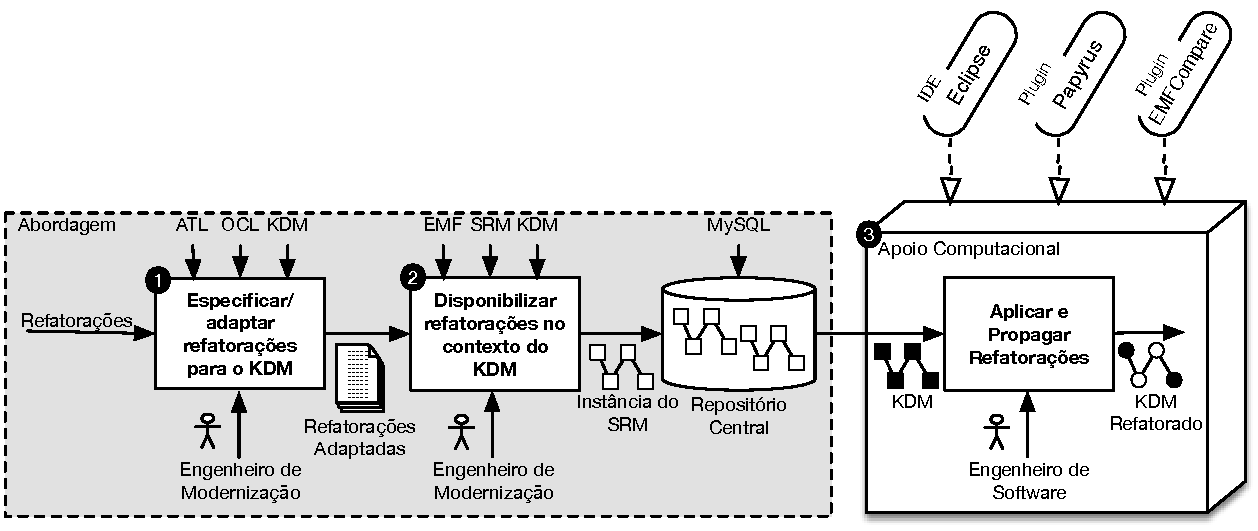
\includegraphics[scale=0.75]{images/Micro_visao_do_doutorado3}
	\fautor
\end{figure}

O passo \ding{183} consiste na disponibilização de refatorações por meio de um metamodelo aqui definido. Esse metamodelo contém metaclasses que permitem armazenar metadados relacionadas com refatorações; por exemplo, o metamodelo permite armazenar os seguintes metadados: o nome da refatoração, sua motivação, autor, pré- e pós-condições e seu mecanismo, etc. É importante salientar que tanto as pré- e pós-condições e os mecanismo das refatorações são disponibilizados no metamodelo por meio de linguagens de transformação e restrições. O objetivo amplo desse metamodelo é permitir e aumentar o reúso de refatorações para um amplo domínio e auxiliar o engenheiro de modernização a definir refatorações representativas em forma de metadados. Em seguida as instâncias desse metamodelo são enviadas para um repositório e são reutilizadas por engenheiros de software por meio de um apoio computacional. 


O apoio computacional (ver Figura~\ref{fig:abordagem_kdm_tese_processo} \ding{184})  também foi implementado para automatizar a atividade de aplicação e reutilização de refatorações em sistemas representados pelo KDM. Para auxiliar o engenheiro de software, as refatorações podem ser aplicadas diretamente em diagramas de classes UML, porém, a refatoração é de fato realizada transparentemente no metamodelo KDM e posteriormente replicada nos diagramas de classes UML. Adicionalmente, após a aplicação de refatorações em sistemas representados pelo KDM é de suma importância manter todos os pacotes/artefatos sincronizados e consistentes. Dessa forma, esse apoio computacional também contém um plug-in responsável por aplicar regras de propagações que são realizadas em instância do metamodelo KDM. O intuito desse plug-in é manter todos os artefatos sincronizados e consistentes de acordo com a refatoração aplicada.


\section{Objetivos}\label{sec:objetivos}

A tese subjacente a este trabalho é de que é possível e benéfico o uso de refatorações para o contexto da ADM, principalmente para o KDM. Nesse contexto, o objetivo geral desta Tese é apresentar uma abordagem para criação e disponibilização de refatorações para o metamodelo KDM, bem como um apoio ferramental que permite aplicá-las em diagramas de classe da UML (ver Figura~\ref{fig:abordagem_kdm_tese_processo}). Mais especificamente pode-se sumarizar os seguintes objetivos:%Para que esse objetivo seja alcançado, os seguintes objetivos específicos devem ser atingidos:

\begin{itemize}

    \item Tornar a criação de refatorações para o metamodelo KDM um processo sistemática e guiado;
    
    \item Viabilizar a disponibilização de refatorações para o metamodelo KDM de forma que possam ser mais facilmente especificadas, disponibilizadas e reusadas;
    
    \item Disseminar conhecimento técnico acerca do desenvolvimento de ferramentas que facilitem o reúso e aplicação de refatorações para o metamodelo KDM em ambientes de modelagem UML; e
    

    \item Propor um metamodelo inicial como uma solução ao \textit{Call for Proposals} do ADM \textit{Refatoring} do OMG. Esse metamodelo possui um conjunto de metaclasses que definem meta-atributos específicos para representar informações (metadados) de refatoração, auxiliando assim o compartilhamento das refatorações de forma intuitiva entre os engenheiros. Além disso, esse metamodelo também possui metaclasses e meta-atributos que representam os mecanismos das refatorações, bem como suas pré- e pós-condições.

	%\item Definir diretrizes para criar refatorações para o metamodelo KDM;
	
	%\item Especificar e criar um metamodelo para auxiliar engenheiros de modernização a compartilhar, criar e reutilizar refatorações no contexto da ADM e KDM;
	
	%\item Elaborar uma linguagem específica de domínio (do inglês - \sigla{DSL}{\textit{Domain-Specific Language}}). Essa DSL possui duas finalidades, a saber: (\textit{i}) auxiliar o engenheiro de modernização a instanciar o metamodelo de refatoração proposto e (\textit{ii}) facilitar a criação de um conjunto de refatorações de forma guiada e automática;
	
	%\item Criar um repositório totalmente integrado com o apoio ferramental para facilitar o compartilhamento e o reúso de refatorações que estão em conformidade com o metamodelo de refatoração proposto; e
	
	%\item Elaborar regras pré-definidas para manter o metamodelo KDM consistente e sincronizado após a aplicar um conjunto de refatorações;
	
    %\item Desenvolver um apoio ferramental totalmente integrado no ambiente de desenvolvimento Eclipse para apoiar a abordagem proposta na Tese.

\end{itemize}




%A tese subjacente a este trabalho é de que é possível e benéfico o uso de refatorações para o contexto da ADM, principalmente para o KDM. %Além disso, pretende-se viabilizar a reutilização e padronizações de refatorações por meio da utilização de um metamodelo de refatorações. Adicionalmente, planeja-se verificar a possibilidade de manter todas as visões do metamodelo KDM sincronizada e consistentes após a aplicação de um conjunto de refatorações. %e de técnicas de propagação de mudanças para manter todas as visões do KDM sincronizadas e consistentes após a aplicação de uma refatoração. 
%Neste contexto, esta tese de doutorado cobre os seguintes aspectos: 


%\begin{itemize}
%	\item Definir diretrizes para criar refatorações para o metamodelo KDM;
	
%	\item Criar regras pré-definidas para manter o metamodelo KDM consistente e sincronizado após a aplicar um conjunto de refatorações;
	
%	\item Especificar e criar um metamodelo para auxiliar engenheiros de modernização a compartilhar, criar e reutilizar refatorações no contexto da ADM e KDM;
	%\item a elaboração de uma linguagem específica de domínio (do inglês - \sigla{DSL}{\textit{Domain-Specific Language}}). Essa DSL possui duas finalidades, a saber: (\textit{i}) auxiliar o engenheiro de modernização a instanciar o metamodelo de refatoração proposto e (\textit{ii}) facilitar a criação de um conjunto de refatorações de forma guiada e automática;
	%\item a definição de um ambiente \emph{Web} para também auxiliar a instanciação do metamodelo de refatoração proposto;
	%\item a concepção de um repositório totalmente integrado com a ferramenta %e com o ambiente \emph{web} 
	%para facilitar o compartilhamento e o reúso de refatorações que estão em conformidade com o metamodelo de refatoração proposto.
	
%	\item Elaborar um apoio ferramental totalmente integrado no ambiente de desenvolvimento Eclipse para apoiar a abordagem proposta na Tese.% que possui três módulos: (\textit{i}) módulo de refatoração; (\textit{ii}) módulo do SRM e (\textit{iii})  %com o objetivo de auxiliar o engenheiro de modernização a aplicar, reutilizar e propagar refatorações de forma gráfica, por meio da utilização de diagramas;
%\end{itemize}


%\section{Contribuições}\label{sec:contribuicoes}

%A principal contribuição dessa Tese de doutorado é entender como refatorações tradicionais, ou seja, refatorações comumente utilizadas em sistemas implementados com o paradigma orientado a objeto, podem ser adaptadas, aplicadas, padronizadas e reutilizadas no contexto da ADM e principalmente para o metamodelo KDM. Em outras palavras, esta pesquisa pode ser entendida como uma incursão inicial para auxiliar o OMG e a ADM na definição de padronizações e soluções ferramentais para facilitar o engenheiro de modernização durante o uso de refatorações para o KDM. Pontualmente, pode-se destacar as principais contribuições dessa tese são:

%\begin{itemize}
%	\item Diretrizes para criar e adaptar refatorações para o metamodelo KDM;
%	\item Regras pré-definidas para manter a instância do metamodelo KDM sincronizado e consistente após a aplicação de refatorações;
%	\item Investigação e definição de um metamodelo para auxilar os engenheiros de modernização a criar, compartilhar e reutilizar refatorações no contexto da ADM e KDM;
%	\item Ambiente para auxiliar o engenheiro de modernização durante a aplicação de refatorações para o metamodelo KDM;
%	\item Definição de uma DSL para auxiliar o engenheiro de modernização a instanciar o metamodelo proposto e facilitar a criação de um conjunto de refatorações de forma guiada e automática;
	%\item a elaboração de um ambiente \emph{Web} para também auxiliar a instanciação do metamodelo de refatoração proposto;
%	\item Concepção de um repositório totalmente integrado com a ferramenta para facilitar o compartilhamento e o reúso de refatorações que estão em conformidade com o metamodelo proposto.
%\end{itemize}
    
\section{Convenções Adotadas nesta Tese}\label{sec:convencoes}

Ao longo desta Tese, \textit{Itálico} é utilizado para dar ênfases, introduzir novos termos e para destacar palavras em inglês. \texttt{Typewriter} é utilizado para operador Java, operador da DSL, palavras-chaves, nome de metaclasses, meta-associação, meta-atributo, nome de métodos, variáveis e URL que aparecem no texto. Símbolos \ding{202}, \ding{203}, \ding{204}, \ding{205} ou \textcircled{a}, \textcircled{b}, \textcircled{c}, \textcircled{d}, são utilizados para chamar a atenção do leitor para informações importantes em figuras e códigos.

\section{Grupo de Pesquisa}

Esse trabalho é uma contribuição para o grupo de pesquisa do Departamento de Ciência de Computação e Estatística do Instituto de Ciências Matemáticas e de Computação (ICMC) da Universidade de São Paulo (campus São Carlos/SP). Além disso, esse trabalho também foi conduzido em parceria com o grupo de pesquisa AdvanSE (\textit{Advanced Research on Software Engineering}), da Universidade Federal de São Carlos (UFSCar). O grupo possui pesquisas em andamento sobre extensões, refatorações, mineração, métricas e validações de arquitetura utilizando a ADM e o metamodelo KDM, as quais o autor desta Tese participa efetivamente.

\section{Estrutura da Tese}

Esta tese está organizada em X\change{mudar} capítulos. No primeiro capítulo estão apresentados o contexto, a motivação, os objetivos, contribuições, convenções adotadas e o grupo de pesquisa do trabalho. 

No Capítulo~\ref{chapter:fundamentacao_teorica} apresenta-se uma revisão dos principais conceitos envolvendo MDD e refatoração com o objetivo de facilitar a compreensão da tese. Além disso, uma contextualização sobre a modernização de sistemas com a utilização dos padrões propostos pelo OMG, ADM e KDM, em que seus conceitos e particularidades são observados. Também é apresentada a ferramenta MoDisco.

%No Capítulo~\ref{chapter:adm_kdm} é ilustrada uma contextualização sobre a modernização de sistemas com a utilização dos padrões propostos pelo OMG, ADM e KDM, em que seus conceitos e particularidades são observados. Também é apresentada a ferramenta MoDisco, utilizada nesta Tese. 

No Capítulo~\ref{chapter:mapeamento_sistematico} é apresentado um mapeamento sistemático que foi realizado com o objetivo de identificar e entender soluções já desenvolvidas sobre ADM e KDM. Além disso, nesse mapeamento também são apresentadas as principais constatações e questões em aberto.

Como apresentado na Figura~\ref{fig:abordagem_kdm_tese_processo} a abordagem proposta nesta Tese contém dois principais passos. O passo \ding{182} é apresentado no Capítulo~\ref{chapter:catalogo_refactoring_KDM} onde são destacadas as diretrizes para adaptar e criar refatorações para o metamodelo KDM. O passo \ding{183} é salientado no Capítulo~\ref{chapter:Toward_a_Refactoring_Metamodel_for_KDM}, o qual apresenta um metamodelo para disponibilizar refatorações e promover o reúso de refatorações no contexto da ADM e KDM. No Capítulo~\ref{chapter:Abordagem_de_sincronizacao} é apresentada uma abordagem denominada KDM-SInc que é utilizada para manter uma determinada instância do metamodelo KDM consistente e sincronizado após a aplicação de refatorações. 

O apoio computacional \ding{184} é apresentado no Capítulo~\ref{chapter:ferramenta_kdm_re}. Esse apoio computacional é denominado KDM-RE e é composto por três plug-ins do Eclipse: (\textit{i}) o primeiro consiste em um conjunto de \textit{Wizards} que apoia o engenheiro de software na aplicação das refatorações em diagramas de classe UML; (\textit{ii}) o segundo consiste em um módulo de propagação de mudanças que permite manter modelos internos do KDM sincronizados e; (\textit{iii}) o terceiro consiste em um apoio à importação e reúso de refatorações disponíveis no repositório.


No Capítulo~\ref{chapter:avaliacao} é mostrado o planejamento, execução e análise dos dados de dois experimentos que visou validar a abordagem desenvolvida nesta Tese.  E por ultimo no Capítulo X\change{mudar} são mostradas as conclusões do trabalho com as principais contribuições, limitações, lições apreendidas, publicações e trabalhos futuros.

%A Tese está estruturada de acordo com a Figura~\ref{fig:structure_these_not_final}

%\begin{figure}[h]
%	\centering
	% Requires \usepackage{graphicx}
	%\caption{Macro visão da abordagem proprosta.}
	%\label{fig:abordagem_kdm_tese_processo}
	%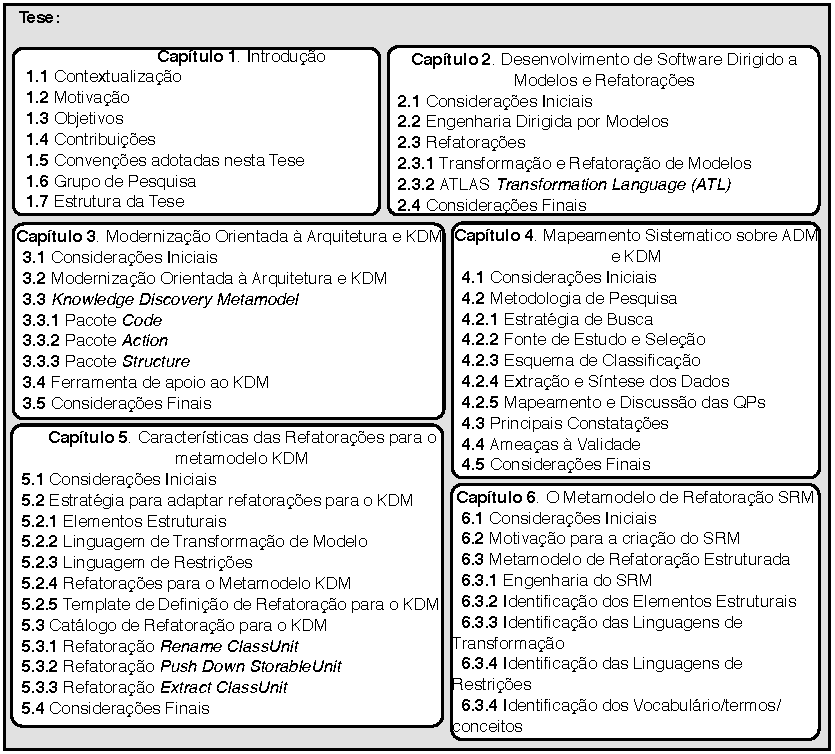
\includegraphics[scale=0.9]{images/PhD_Structure_Figure}
	%\fautor
%\end{figure}